\documentclass[aps,reprint,superscriptaddress,10pt]{revtex4-2}
\usepackage{kotex}
\usepackage[HWP]{dhucs-interword}
\usepackage[dvips]{color}
\usepackage{graphicx}
\usepackage{bm}
\usepackage{amsmath}
\usepackage{tikz}
\usepackage{mhchem}
\usepackage{booktabs}
\usepackage{multirow}
\usepackage{array}
\usepackage{tikz}
\usepackage{tabularx}

\begin{document}
\title{응집물질물리실험 결과보고서 \\
\small 실험주제 : Hall effect}

\author{HuiJae-Lee}\email{hjlee6674@inha.edu}
\affiliation{Physics Department, Inha University}

\date{\today}


\begin{abstract}
반도체에 걸리는 홀 전압의 크기가 외부 자기장에 비례하여 커지고 반도체에 흐르는 전류의 크기에
대해서도 비례하여 증가함을 관찰하였다. 또한 외부 자기장과 홀 전압으로부터 시료의 홀 계수를
구하였다.
\end{abstract}
 
 \maketitle
 
 \section{Process}
 \begin{itemize}
     \item[1.]
     가우스미터를 통해 전자석의 자기장 크기를 전류의 값으로 치환한다.
     \item[2.] 전자석의 자기장 세기를 6000 G까지 100 G씩 올려가며 가우스미터의 
     전류 값을 기록한다.
     \item[3.] p형 반도체 샘플이 전자석의 중앙에 위치하도록 조정하고 홀 전압 측정 장치에 
     연결한 후, 측정 장치의 off set을 0으로 설정한다. 
     \item[4.] 샘플에 흐르는 전류를 측정할 값(2 mA, 4 mA, 6 mA)에 맞춘 후, 자기장을
     올려가며 홀 전압을 측정한다.
     \item[5.] 샘플을 n형 반도체로 교체하여 과정 3, 4를 반복한다.
   \end{itemize}
\section{Result}
\subsection{p-type}
\begin{figure}[htbp]
  \centering
  \vspace{-0.5cm}
  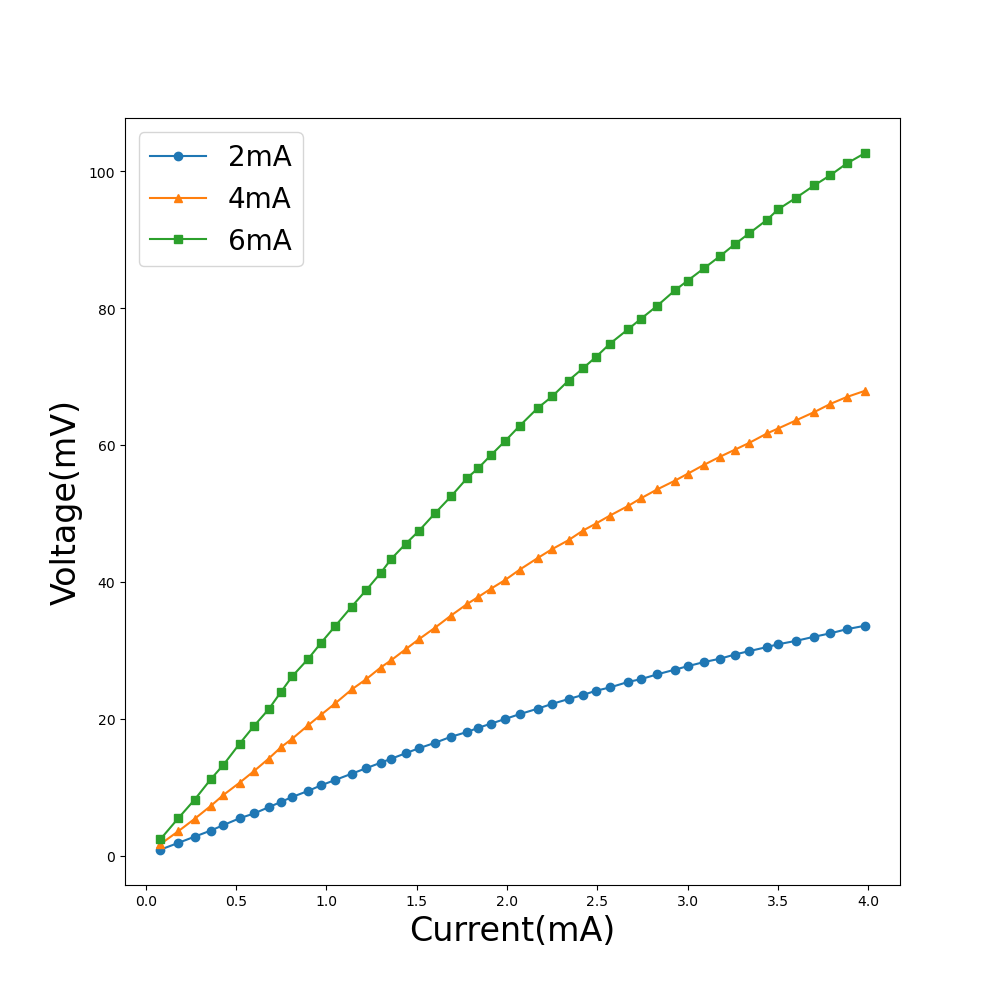
\includegraphics[scale = 0.3]{Hall_p.png}
  \caption{전자석에 흐르는 전류에 따른 p형 반도체의 홀 전압 그래프}\label{fig:p}
\end{figure}
p형 반도체의 경우, offset을 0으로 잘 설정하여 실험을 진행하였다.


\subsection{n-type}
\begin{figure}[htbp]
  \centering
  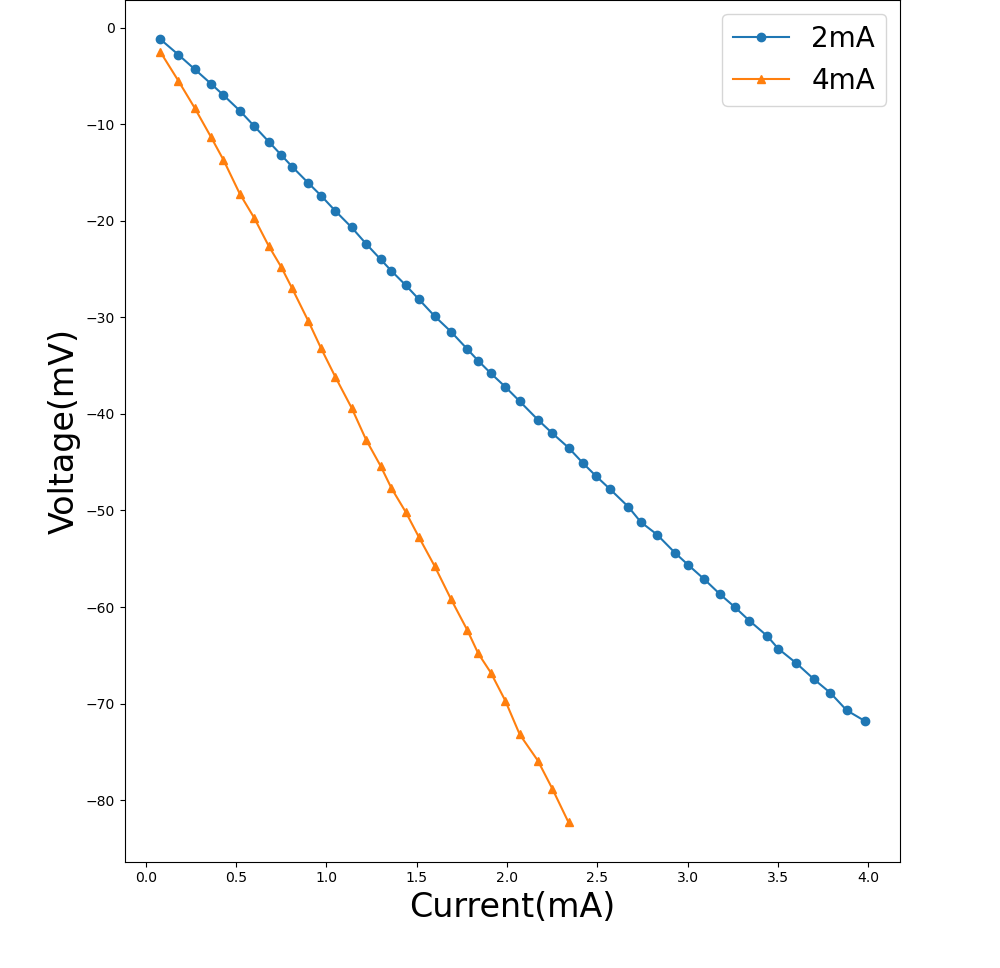
\includegraphics[scale = 0.3]{Hall_n.png}
  \caption{전자석에 흐르는 전류에 따른 p형 반도체의 홀 전압 그래프}\label{fig:n}
\end{figure}
n형 반도체의 경우 offset이 잘 설정되지 않아 반도체에 2 mA가 흐르는 조건에서 자기장이 0 G일 때
홀 전압이 $-37.5$ mV, 4 mA가 흐르는 조건에서 자기장이 0 G일 때 홀 전압이 $-115.3$ mV 만큼 걸리는
것을 측정하였다. 홀 전압을 측정하는 기기가 200 mV 이상의 전압을 측정하지 못해 4 mA가 흐르는
조건에서 자기장이 3000 G 이상일 때 홀 전압을 측정하지 못하였고 6 mA가 흐르는 조건에서 홀 전압을
전혀 측정하지 못하였다.
\newpage
\section{Analysis}
실험에 사용한 시료의 두께는 0.05 cm로 홀 계수 $R_H$를 다음의 공식으로부터 구할 수 있다.
\begin{align}\label{eq:1-1}
  R_H = \frac{dV_H}{IB}
\end{align}
$d,\,V_H,\,I,\,B$는 각각 시료의 두께, 홀 전압, 시료에 흐르는 전류, 외부 자기장이다.
\subsection{p-type}
\begin{figure}[htbp]
  \centering
  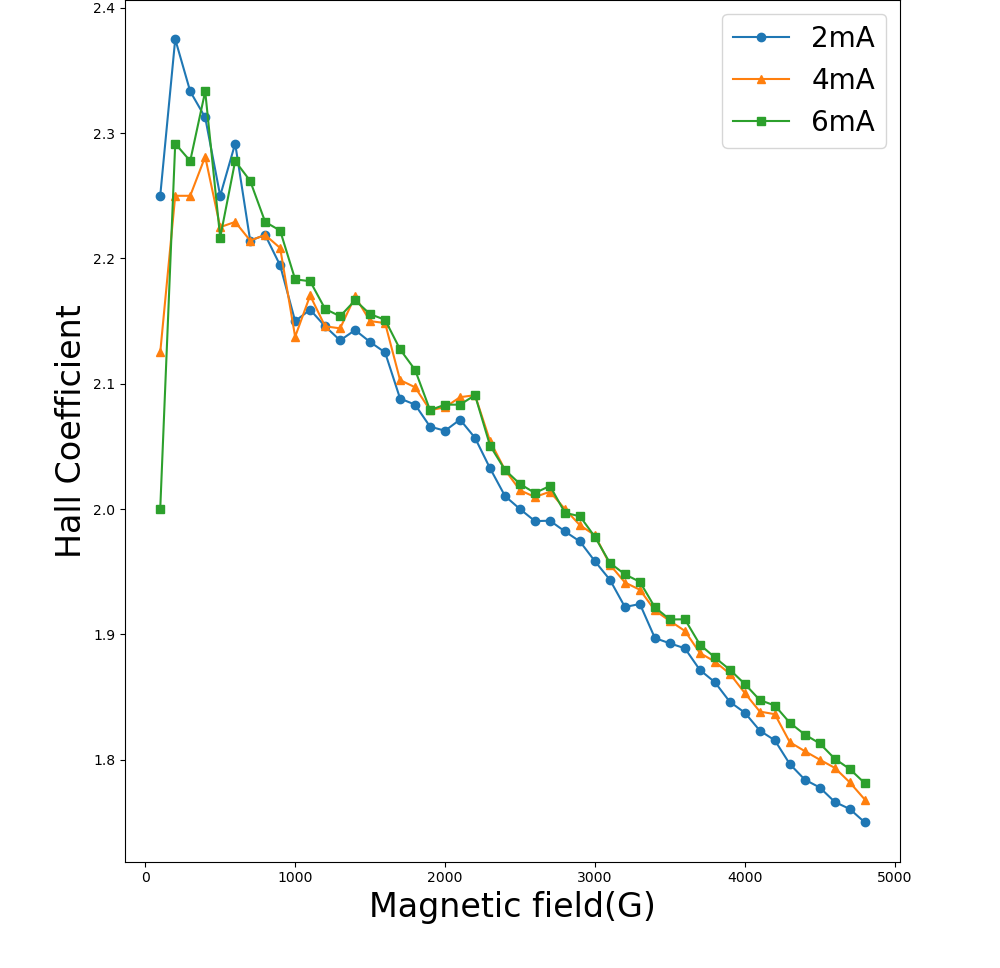
\includegraphics[scale = 0.3]{co_p.png}
  \caption{외부 자기장에 따른 p형 반도체의 홀 계수}\label{fig:co_p}
\end{figure}
실험으로부터 얻은 측정값(외부 자기장, 홀 전압)으로부터 구한 외부 자기장에 따른 
p형 반도체의 홀 계수를 FIG.~\ref{fig:co_p}과 같이 그래프로 그릴 수 있다. 반도체에 흐르는
전류에 따른 홀 계수의 평균값은 다음과 같다.
  \begin{table}[htbp]
    \centering
    \begin{tabular}{ c|c } 
      \hline
      \hline
      Current & Average Hall Coefficient \\
      \hline
      2 mA & 2.019940377$\times 10^{-6}$ \\ 
      
      4 mA & 2.024756306$\times 10^{-6}$ \\ 
      
      6 mA & 2.032621037$\times 10^{-6}$ \\ 
      \hline
      \hline
    \end{tabular}
    \caption{p형 반도체에 흐르는 전류에 따른 홀 계수의 평균값}
    \end{table}

  반도체에 흐르는 전류가 높을 수록 홀 계수가 평균적으로 증가하였고, 반도체에 흐르는 전류에
  관계없이 외부 자기장이 클 수록 홀 계수가 낮아지는 양상을 확인할 수 있었다.
\subsection{n-type}

\begin{figure}[htbp]
  \centering
  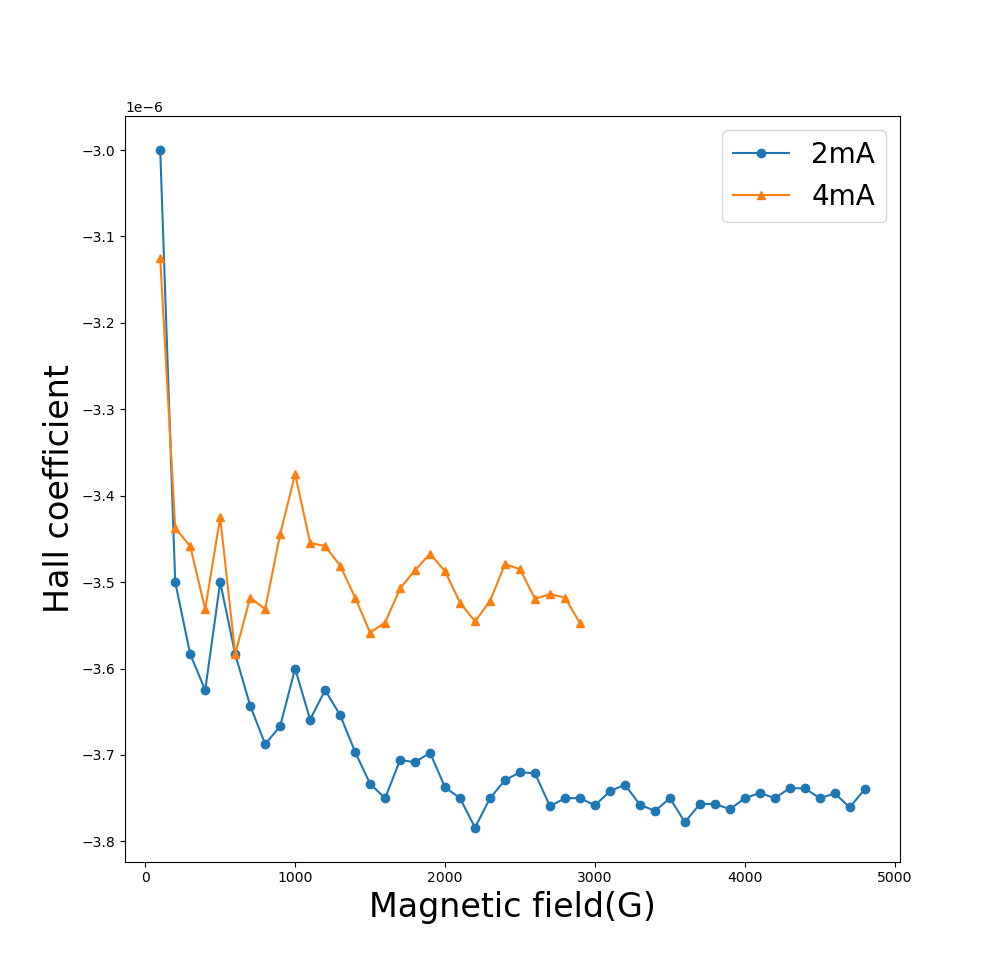
\includegraphics[scale = 0.3]{co_n.png}
  \caption{외부 자기장에 따른 n형 반도체의 홀 계수}\label{fig:co_n}
\end{figure}

p형 반도체의 경우와 마찬가지로 외부 자기장에 따른 
n형 반도체의 홀 계수를 FIG.~\ref{fig:co_n}과 같이 그래프로 그릴 수 있다. 위에서 언급하였듯이 
n형 반도체의 경우 4 mA가 흐르는 조건에서 홀 전압을 2900 G 까지만 측정할 수 있었고
6 mA가 흐르는 조건에서 홀 전압을 측정할 수 없어 FIG.~\ref{fig:co_n}에는 2개의 그래프가 그려져
있다. 반도체에 흐르는 전류에 따른 홀 계수의 평균값은 다음과 같다.
\vspace{0.2cm}
  \begin{table}
    \begin{tabular}{ c|c } 
      \hline
      \hline
      Current & Average Hall Coefficient \\
      \hline
      2 mA & -3.694702113$\times 10^{-6}$ \\ 
      4 mA & -3.484390053$\times 10^{-6}$ \\ 
      \hline
      \hline
    \end{tabular}
    \caption{n형 반도체에 흐르는 전류에 따른 홀 계수의 평균값}
    \end{table}


n형 반도체의 경우 홀 계수의 평균값의 차가 p형 반도체의 경우보다 10배 가까이 크게 나타났다.
\section{Conclusion}
우선 가우스미터를 통해 전자석의 자기장 크기를 전류값으로 치환하였을 때 전류값은 자기장에
거의 선형적인 모습으로 나타났다(FIG.~\ref{fig:compare}).
\begin{figure}[htbp]
  \centering
  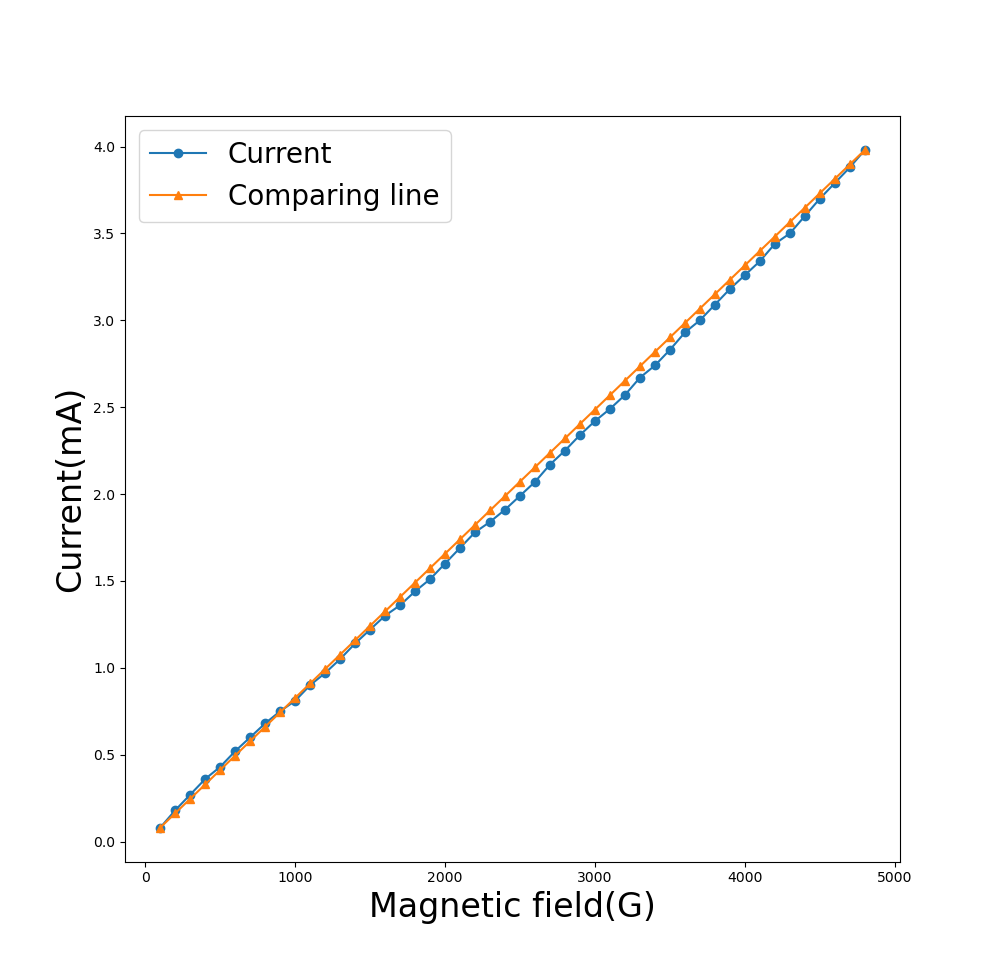
\includegraphics[scale = 0.3]{compare.png}
  \caption{전자석의 자기장 크기에 대한 전류 그래프}\label{fig:compare}
\end{figure}
따라서 p형 반도체와 n형 반도체의 홀 전압 그래프(FIG.~\ref{fig:p}, FIG.~\ref{fig:n})는
자기장에 대한 홀 전압 그래프로 보아도 무방하다.
\begin{itemize}
  \item[1. ] 홀 전압 그래프를 보았을 때 p형과 n형의 경우 모두 홀 전압이 자기장에 대해
  선형적으로 증가하였다가 자기장이 커짐에 따라 홀 전압의 증가 추세가 감소하는 것으로
  보여진다. 이는 반도체 시료를 전자석의 정확한 중앙에 위치시키지 않아 전류에 따른
  자기장이 반도체가 위치한 부분에서 균일하지 않게 증가하였기 때문이라고
  추측할 수 있다.
  \item[2. ] p형 반도체의 홀 계수는 반도체에 흘려준 전류가 높아질 수록 그 평균값이 대략
  0.5\% 높게 계산되었다. 흘려준 전류에 상관없이 홀 계수는 자기장이 증가할 수록 작아지는
  양상을 보였고 이는 1에서 언급한 홀 전압-자기장의 비선형성 관계에 의한 것이다.
  식~\eqref{eq:1-1}에 의하면 홀 계수는 홀 전압-자기장 그래프의 기울기에 비례하는데
  FIG.~\ref{fig:p}에서 볼 수 있듯이 그래프의 기울기는 자기장이 높아질 수록 감소한다.
  이로 인해 홀 계수가 작아지는 양상을 보였다.
  \item[3. ] n형 반도체의 홀 계수는 반도체에 흘려준 전류가 높아졌을 때 그 평균값이 대략
  10\% 높게 계산되었다. 이는 p형 반도체의 증가치에 비해 현저히 큰 값이다. 홀 계수가 
  작아지는 양상을 p형 반도체와 일치하였으며 2에서 분석한 p형 반도체의 경우와 홀 계수가
  감소한 이유가 같다. 반도체에 흘려준 전류값이 달라졌을 때 홀 계수가 p형 반도체에 비해 
  크게 변한 이유는 반도체에 흘려주는 전류를 바꾸면서 반도체의 위치 또한 재조정 시켰기
  때문이라고 생각한다. 반도체의 위치가 달라졌으므로 반도체에 작용하는 자기장의 크기가
  달라져 같아야할 홀 계수가 달라진 것이다.
\end{itemize}



% \nocite{*} 
% \bibliography{ref}



%\begin{thebibliography}{9}
%\end{thebibliography}

\vfill
\end{document}